\chapter{背景知识与相关工作}

\section{模型、计算图与设备}
% 介绍一些专业术语
本节介绍一些与本文工作相关的术语和背景知识。
包括对神经网络模型、计算图以及神经网络训练设备的介绍。
\subsection{模型}
本文中所提到的模型指的是深度神经网络模型(Deep Neural Network, DNN)。
深度神经网络模型来自机器学习的分支领域深度学习,深度学习包括深度神经网络,深度信念网络,深度强化学习等。
深度神经网络模仿人脑中神经元的运作方式,通过激活函数连接模拟神经元。
多层感知机(Multilayer Perceptron, MLP) \upcite{mlp}是最简单的神经网络。
深度神经网络包含一个输入层,一个输出层和至少一层的隐藏层(Hidden Layer)。
每一层都由若干神经元组成,输入数据按照一定规则和神经元的参数进行运算,得到该神经元的输出。
输出经过非线性激活函数后,再作为下一层神经元的输入。
非线性激活函数的存在可以让深度神经网络以任意精度拟合任何函数,为复杂的非线性系统提供建模能力 \upcite{ml-book}。

深度神经网络的建模效果取决于神经元的参数,神经元的参数使用反向传播算法 \upcite{bp}进行训练更新。
反向传播算法的主要过程是首先通过前向传播获取网络的输出,然后选择损失函数(Loss Function),计算网络输出和真实标签的损失(Loss)。
然后反向传播,逐层求解神经元的参数关于损失的梯度,根据选用的优化方法进行梯度下降,更新参数,完成一次训练。
\begin{equation}
	\label{eq:bp}
	W_{i,j}(t+1) = W_{i,j}(t) + \eta \frac{\partial Loss}{\partial W_{i,j}(t)}
\end{equation}

公式 \ref{eq:bp}展示了反向传播算法中一次参数更新的过程。
其中的$Loss$ 代表损失函数计算出的损失,交叉熵损失函数 \upcite{cross-entropy}是一种常用的用于分类任务的损失函数。

\subsection{计算图}
% 深度学习框架的发展

为了帮助深度学习开发者更好的进行模型开发工作,越来越多的开源深度学习框架被设计出来,例如Google开源的Tensorflow \upcite{tensorflow},Facebook开源的PyTorch \upcite{pytorch}等。
随着深度学习框架多年的发展,从方便开发者的角度出发,框架提供更多高层的抽象封装,开发者可以使用高层的应用程序接口迅速搭建自己的模型,而不需要深入到模型底层,处理神经元之间的连接。
而神经元与神经元之间的连接所构成的图,就是深度学习中模型的计算图(Computational Graph)。

最初,开发者需要自己定义计算图中的节点,以及节点与节点之间的连接。
以Tensorflow的发展历程来看,在Tensorflow 1.x版本中,开发者需要手动定义计算图,因此开发一个复杂的模型的十分繁琐,而且静态的计算图给开发调试带来了很多不便。
而在Tensorflow 2.x版本中,则引入了动态图的设定,计算图隐藏在代码中,大大简化了模型的开发流程。
下面是在Tensorflow 1.x和2.x中定义 $a+b$ 的代码片段。

\begin{lstlisting}[language=Python, caption={静态图与动态图的比较}]
# tf 1.x: 手动定义计算图
import tensorflow as tf
a = tf.placeholder(tf.float32, name='var_a')
b = tf.placeholder(tf.float32, name='var_b')
add_op = tf.add(a, b, name='var_c')
sess = tf.InteractiveSession()
init = tf.global_variables_initializer()
sess.run(init)
res = sess.run(add_op, feed_dict={a:2., b:4.,})

# tf 2.x: 自动生成计算图
import tensorflow as tf
a = tf.constant(2.)
b = tf.constant(4.)
print('a+b=', a+b)
\end{lstlisting}


% 模型和计算图的关系
随着框架的发展,已经不需要静态定义完整的计算图,框架可以从开发者的模型定义中动态生成计算图。
在PyTorch和Tensorflow 2.x中,用户通过描述模型的计算过程来定义模型。
计算图则在模型训练时由框架从计算过程的定义中动态生成。
如图 \ref{fig:graph} 所示,这种动态生成计算图的方式帮助开发者屏蔽了底层的细节,提升开发效率,但是也为运行时模型划分带来了困扰。
计算图对用户来说是不透明的,所以从开发者层面无法控制计算图如何被放置,这也是本文工作尝试去解决的问题,
即针对动态图框架,自动的对计算图进行划分。

\begin{figure}[htbp]
	\centering
	\begin{minipage}[b]{0.66\textwidth}
	  \lstinputlisting[language=Python]{figure/2-background/graph.py}
	\end{minipage}
	\hfill
	\begin{minipage}[b]{0.3\textwidth}
	  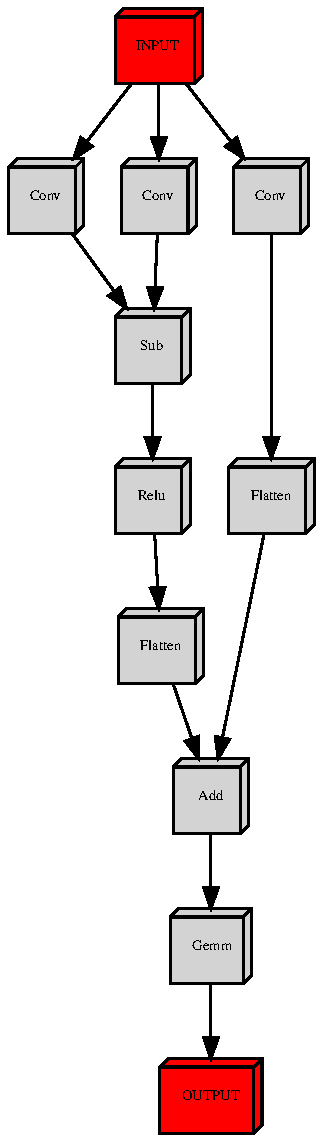
\includegraphics[height=8cm]{./figure/2-background/graph.pdf}
	\end{minipage}
	\caption{模型定义和底层计算图}
	\label{fig:graph}
\end{figure}

\subsection{设备}
% GPU设备的特点
% % 和CPU的区别
% % 内存模型特点
% % 使用CUDA和CUDNN进行计算
% % GPU之间的连接方式介绍, 同个机器上 PCIe, NVLink, 跨节点使用NCCL
本文中所提到的设备特指GPU(Graphics Processing Unit),也就是图形处理器。
最初,GPU主要用于绘制图像和渲染图形,随着高性能计算需求的发展,GPU也发展出了其他的用途,例如用于深度学习中的模型训练、大规模并行处理、以及其他更为严苛的工作负载。
与CPU相比,GPU具有更多的处理单元。
CPU适用于通用的工作负载,特别是对于执行延迟敏感以及对单核性能要求更高的工作负载。
CPU将它数量相对较少的处理器核心集中用于处理单个任务,这让CPU更适合处理串行计算的任务。

通过单指令多数据技术(Single Instruction Multiple Data, SIMD),GPU中的多个计算单元可以同时在不同数据上执行同一条指令,这种架构让GPU适用于处理多维向量数据。
同时也让GPU特别适用于进行并行计算。图 \ref{fig:cpu-gpu}展示了CPU和GPU架构上的区别。
GPU对于高维向量的计算效率也受到了深度学习研究者的青睐,越来越多的深度学习负载运行在GPU上,使用GPU对神经网络和大量高维数据集进行深度学习训练已经成为了深度学习领域的最佳实践。
而GPU厂商也在积极为深度学习提供支持,由Nvidia® 开源的 CUDAToolkit \upcite{cuda}是目前最流行的GPU编程框架,可以让开发者使用GPU来加速自己的程序中的并行计算部分。

因为GPU通常需要处理大量高维数据,因此读取数据的带宽和数据加载的时延都具有较高的要求。
所以和CPU相比,GPU拥有自己独立的内存,通常称之为显存(Video Memory)。
以Nvidia® V100 GPU为例,它具有900GB/s的显存带宽,而通常的内存带宽只有20GB/s。
但是显存的容量也限制了设备能够运算的数据规模,顶级GPU通常有24~80GB的显存,但是与服务器内存相比,在面对大量数据时,仍然无法满足需求,当可用显存无法满足需求时,通常会引发内存溢出错误(Out of Memory, OOM)。
如何利用多个设备的组合来满足超大模型对的显存需求,也是本文的工作之一。

\begin{figure}[h]
	\centering
	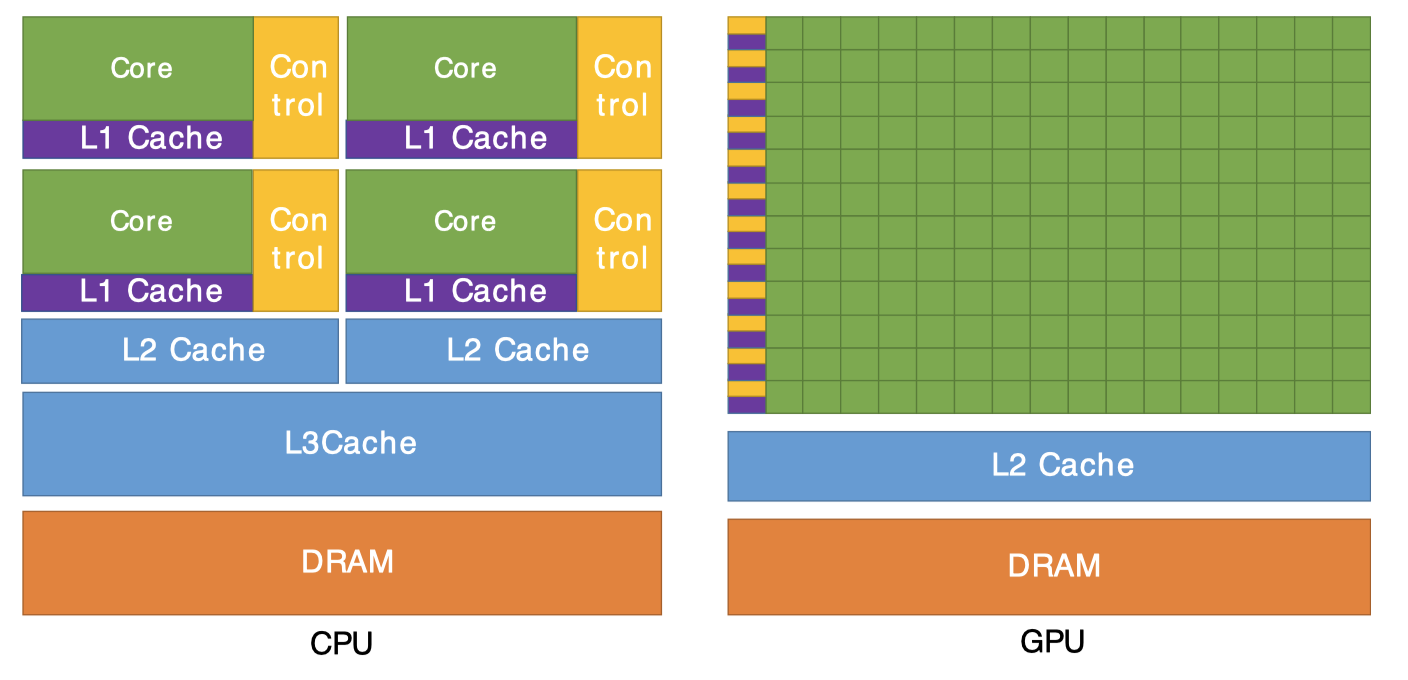
\includegraphics[width=0.85\textwidth]{figure/2-background/cpu-gpu.png}
	\caption{CPU和GPU的架构}
	\label{fig:cpu-gpu}
\end{figure}

受限于单个设备的显存容量和计算能力,多个GPU也常在一起使用,进行并行计算和分布式计算。
在分布式计算过程中,GPU不仅需要处理自己的数据,通常也需要和其他GPU进行数据传输和交换。
使用传统的共享内存或者Socket的方式进行数据传输无法满足GPU之间通信速度的需求。
Nvidia® 开发的NCCL(Nvidia Collective Communication Library) \upcite{nccl}通信库提供了GPU之间进行通信的原语。
NCCL不仅提供了用于点对点通信的原语\texttt{send},\texttt{recv},还提供了例如\texttt{gather},\texttt{broadcast}等集合式通信原语,满足多节点的通信需求。

NCCL从软件层面提供了GPU设备之间通信的功能。在硬件层面,GPU之间有多种通信链路,如图 \ref{fig:gpu-commu} 所示,在计算集群中,GPU之间的通信链路可能有很多不同类型。
在同一个服务器的上的GPU之间可以通过PCIe swtich,也可以使用专有的GPU通信设备NVLink或者NV-Switch \upcite{nvlink}进行通信。
在跨节点通信方面,在非专用集群中,10~25Gbps Ethernet Network Interface Controller(NIC) 仍然是主流选择。
在对通信性能要求较高的场景中,使用 Ehternet NIC则无法满足需求,因此Remote Direct Memory Access(RDMA) \upcite{rdma} 技术被提出。
RDMA协议允许通信实体绕过操作系统内核而直接访问内存中的数据,可以大大提高通信带宽和降低通信延迟,使用RDMA协议的通信设备,例如 Infiniband \upcite{infiniband},可以达到100Gbps的通信带宽。

在分布式计算中,GPU与GPU之间异构的通信链路为系统的设计和工作负载的分发带来了很多挑战。
在分布式深度学习训练中,设备与设备之间需要传递大量的数据。
如果在进行工作负载分发时没有充分考虑集群中通信链路的异构性,则容易导致通信瓶颈的出现,继而影响整个任务的运行效率。
\begin{figure}[h]
	\centering
	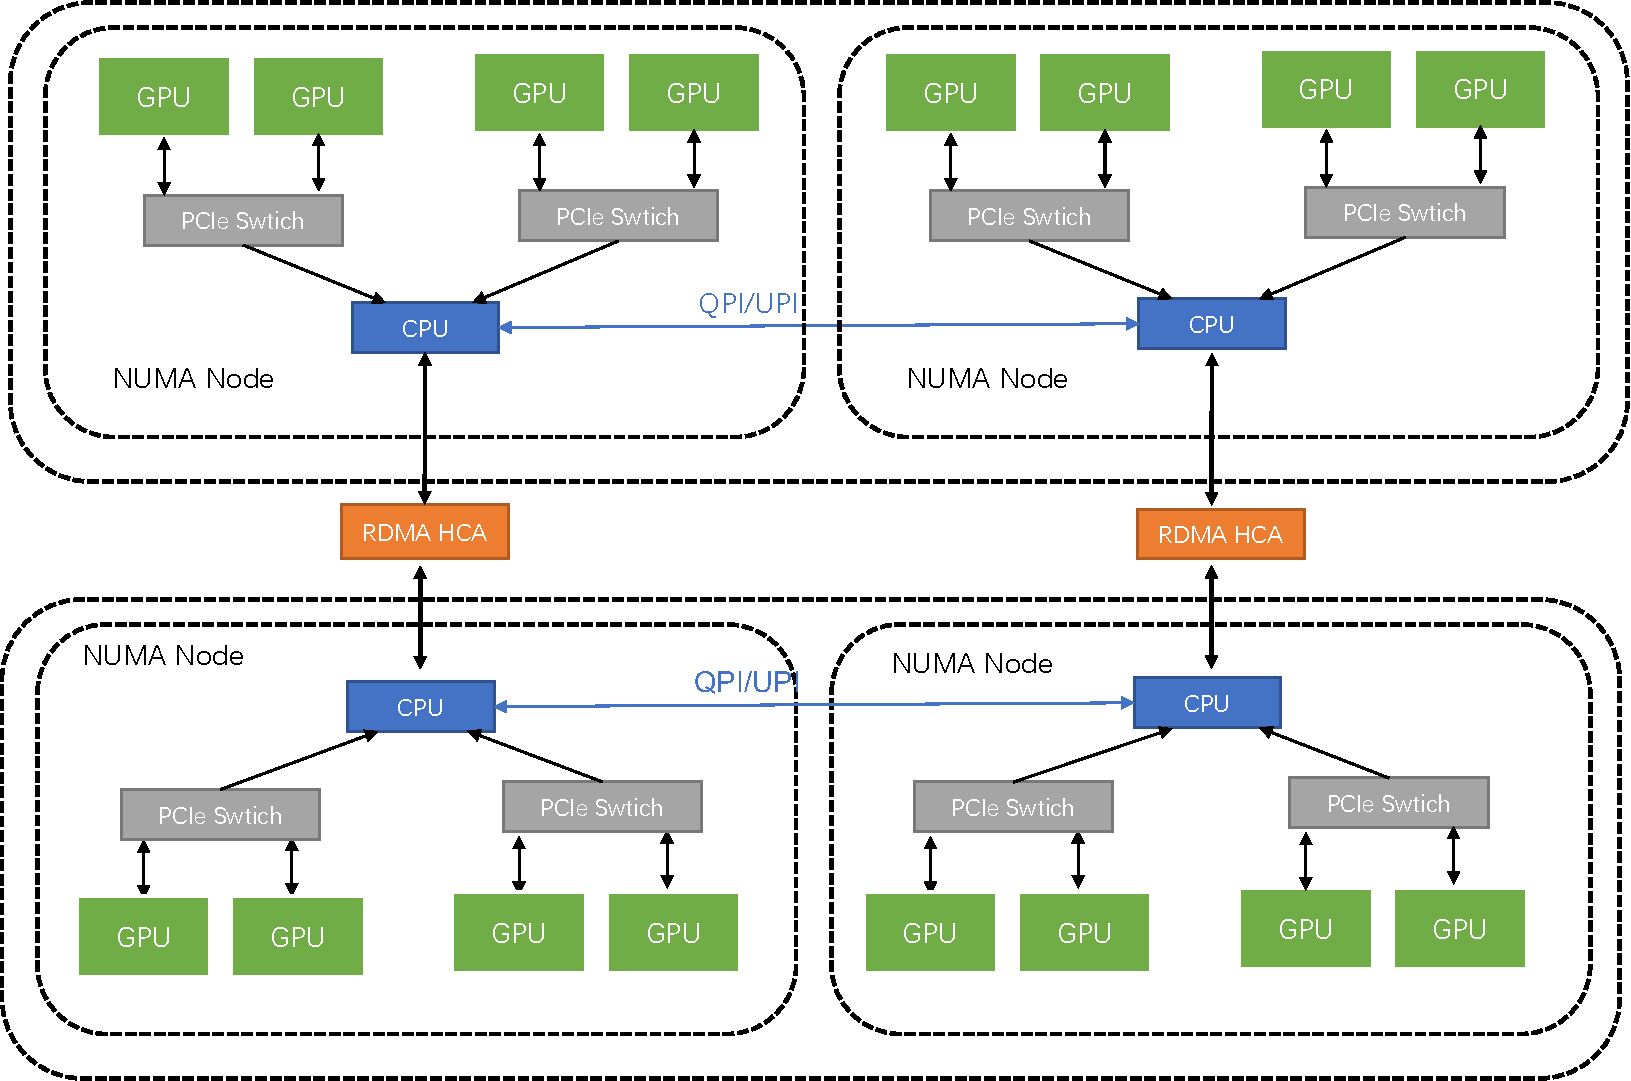
\includegraphics[width=0.9\textwidth]{figure/2-background/commu.pdf}
	\caption{集群中GPU之间通信链路}
	\label{fig:gpu-commu}
\end{figure}

\section{分布式深度学习}
在大数据时代,随着新的应用场景的出现,有更多的数据被收集,而深度学习技术也被广泛的应用在分析数据,构建人工智能应用中, 例如自动驾驶系统 \upcite{self-driving1,self-driving2},AI智能编程助手Copilot \upcite{copilot}等。
目前,面对数据量的增加和模型复杂度的提升,算法研究者们面对的一个重要问题就是如何使用分布式的方式,加速深度神经网络的训练流程。另一方面,模型本身的容量也可能超过单个设备的限制,因此,需要考虑将模型划分到多个设备上,来缓解单个设备的容量不足的问题。
数据并行化(Data Parallelism) \upcite{dp} 与模型并行化(Model Parallelism) \upcite{mp} 分别是分布式深度学习的两种常用的模式,图 \ref{fig:dp-mp} 展示了这两种并行化模式的结构。
% 图 + caption说明
\begin{figure}
	\centering
	\caption{分布式深度学习的两种模式}
	\label{fig:dp-mp}
	\begin{subfigure}[b]{0.4\textwidth}
		\centering
		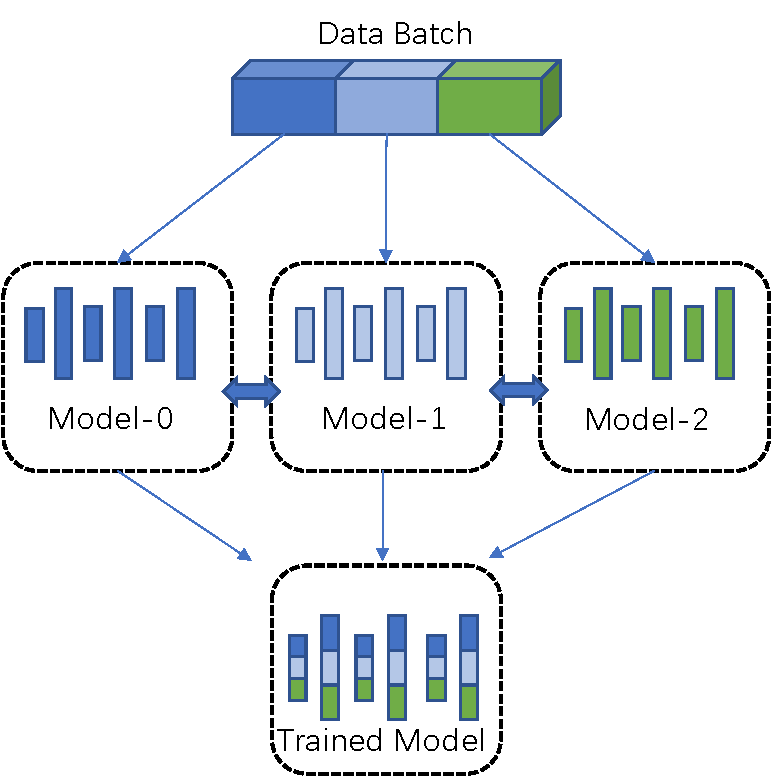
\includegraphics[width=0.85\textwidth]{figure/2-background/dp.pdf}
		\caption{数据并行化}
	\end{subfigure}
	\begin{subfigure}[b]{0.4\textwidth}
		\centering
		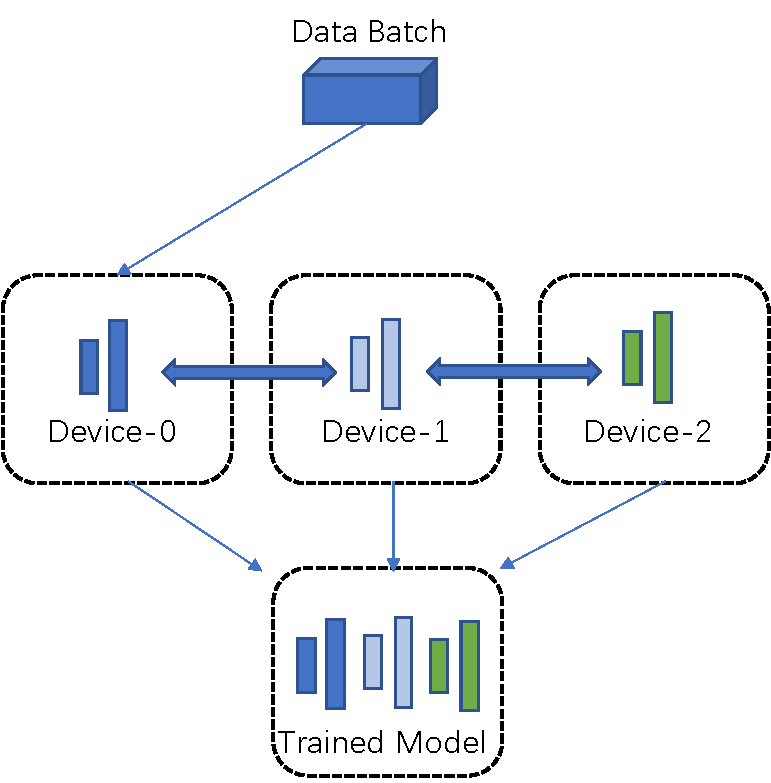
\includegraphics[width=0.85\textwidth]{figure/2-background/mp.pdf}
		\caption{模型并行化}
	\end{subfigure}
	\caption*{a. 数据并行化从训练数据的层面进行并行化,同时训练多个完整的模型副本,每个模型副本使用数据集的一个子集;b. 模型并行化从模型的层面进行并行化,模型并行化将单个模型划分到多个设备上,每个设备负责一部分模型的训练。}
\end{figure}

\subsection{数据并行化}
% 数据并行化的思想
% 数据并行化的两种经典结构 Ring和PS
尽管GPU等专用设备可以加速模型的训练,但是单个设备的算力和容量有限。
利用多个设备通过分布式的方式进行模型训练是加速训练过程的有效方式,多种分布式训练架构被设计出来。
为了应对海量训练数据,数据并行化技术被提出,数据并行化的主要思想为使用多个设备同时训练同一个模型的多个副本。
每个副本使用数据集的一个子集进行训练。
不同的副本周期性通过集合式通信(Collective Communication)进行同步。
在实践中,通常使用数据采样器,采样出一个较大的数据批,然后将数据批按照模型的副本数目进行等分,可以得到多个小数据批。
每个模型副本使用一个小数据批,使用反向传播算法进行训练,然后通过集合式通信,将所有的模型副本的参数梯度求和平均。
每个模型副本使用平均后的梯度来更新模型。

\begin{equation}
	\label{eq:dp}
	\begin{aligned}
		\frac{\partial Loss}{\partial W_{i,j}(t)} =& \frac{\partial \frac{1}{n} \sum_{k=1}^{n} f(x_k, y_k)}{\partial W_{i,j}(t)} = \frac{m_1}{n}\frac{\partial \frac{1}{m_1} \sum_{k=1}^{m_1} f(x_k, y_k)}{\partial W_{i,j}(t)} + \cdots + \frac{m_p}{n}\frac{\partial \frac{1}{m_p} \sum_{k=1}^{m_p} f(x_k, y_k)}{\partial W_{i,j}(t)} \\
		=& \frac{m_1}{n} \frac{\partial L_1}{\partial W_{i,j}(t)} + \cdots + \frac{m_p}{n} \frac{\partial L_p}{\partial W_{i,j}(t)} \\
		=& \frac{1}{p} \sum_{k=1}^{p} \frac{L_k}{\partial W_{i,j}(t)}
	\end{aligned}
\end{equation}

如公式 \ref{eq:dp}所示,
对于大小为$n$的数据批,将其分为$p$份,每份的大小为$m_i,\ 0\le i\le p-1$,每份数据都交给某个设备进行训练。
当满足$m_i=\frac{n}{p}$时,原始数据批关于参数的梯度等于每个小数据批关于参数的梯度的均值。
数据并行化中的关键步骤在于每次反向传播结束后,对不同模型副本的参数梯度进行同步。
参数梯度同步的目的是让模型副本之间共享彼此当前的训练的结果。
从参数梯度同步的架构上,主流的架构有参数服务器架构(Parameter Server, PS) \upcite{ps} 和All-Reduce \upcite{ring} 架构。

\begin{figure}
	\centering
	\begin{subfigure}[b]{0.48\textwidth}
		\centering
		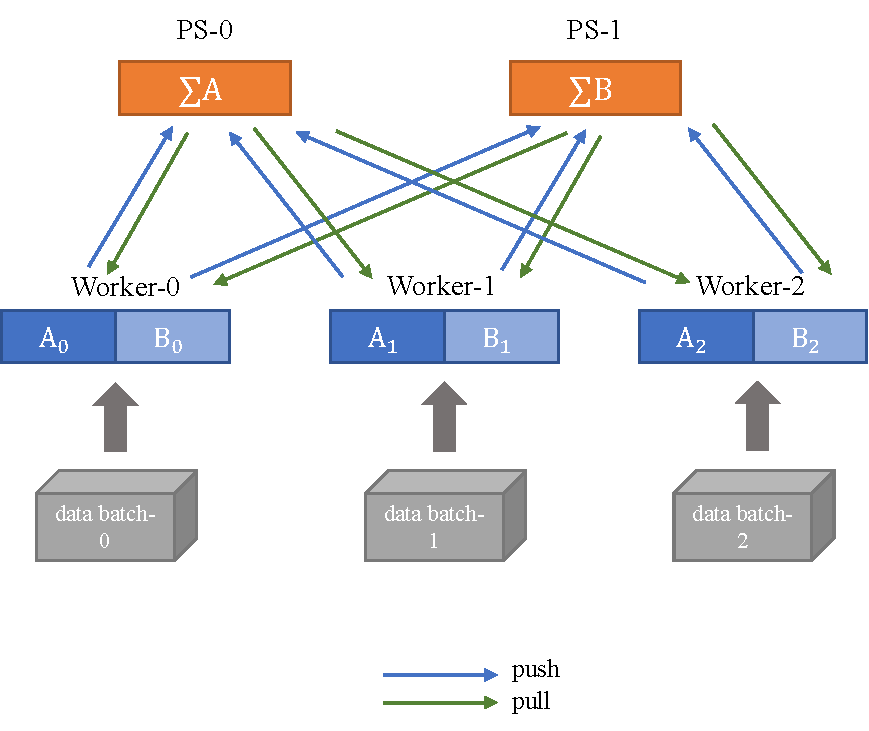
\includegraphics[width=0.95\textwidth]{figure/2-background/ps.pdf}
		\caption{参数服务器架构}
		\label{fig:ps}
	\end{subfigure}
	\begin{subfigure}[b]{0.45\textwidth}
		\centering
		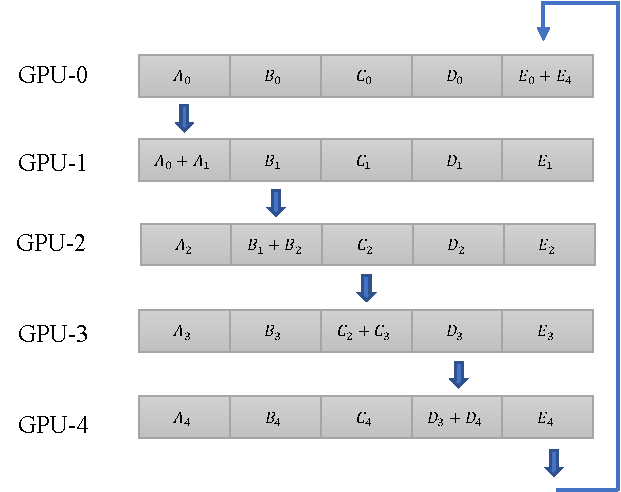
\includegraphics[width=0.95\textwidth]{figure/2-background/ring.pdf}
		\caption{Ring All-Reduce架构}
		\label{fig:ring}
	\end{subfigure}
	\caption{参数服务器架构 vs Ring All-Reduce架构}
	\label{fig:ps-ring}
\end{figure}

\begin{itemize}
	\item \textbf{参数服务器架构}: 参数服务器架构 \upcite{ps} 是最经典的分布式深度学习架构。如图 \ref{fig:ps} 所示,这种架构中,参与训练的节点被从逻辑上划分为了工作节点(Worker Node)和参数服务器节点(PS Node)。
	参数服务器节点的作用是存储模型的参数状态。
	工作节点的职责是进行模型的训练。
	当工作节点完成本地模型的训练后,会将本地最新的模型参数推送到参数服务器。
	参数服务器在接收到工作节点推送的模型参数后,会更新其存储到全局参数。
	然后工作节点再从参数服务器上拉取模型的全局参数。
	参数服务器可以有多个,每个参数服务器存储一部分模型。
	这种架构的优点在于工作节点和参数服务器节点的数量可以根据具体的硬件环境灵活调整,这让参数服务器架构拥有灵活的扩展能力。
	缺点在于参数服务器架构是中心化的架构,通信在参数服务器节点和工作节点之间频繁发生,而参数服务器节点往往需要同时和多个工作节点进行通信,容易导致通信瓶颈的产生。
	在参数服务器架构的基础上,衍生出多种改进版本。如BytePS \upcite{byteps},ElasticPS \upcite{elasticps},ParameterHub \upcite{pshub}等。

	\item \textbf{All-Reduce架构}: 以Ring All-Reduce \upcite{ring} 为代表的All-Reduce架构是一种去中心化的参数同步架构。
	如图\ref{fig:ring} 所示,在All-Reduce架构中,参与训练的计算节点被组织成为一个逻辑环。
	环上的每个节点都有唯一的前驱和后继,通信只发生在节点和前驱/后继之间。
	由于环上所有节点都是处于对称地位,所以每个节点的通信量是相同的,这也避免了参数服务器架构中的通信瓶颈的出现。
	每个节点在训练完成后,都将本地的模型参数分块后,在环上传递给自己的后继。
	在节点数目为$n$时,经过$2(n-1)$ 次通信就可以完成参数的同步。

	\item \textbf{Peer-to-Peer 架构}: 相比于对架构有严格限制的参数服务器架构和All-Reduce架构,Peer-to-Peer 架构采取了一种完全分布式的方式。每个工作节点都有完整的模型副本,工作节点之间直接进行点对点通信。
	这种方式具有更高的可扩展性,而且可以很好的处理分布式系统中的单点故障问题。
	受到这种思想的启发,Gossip Learning \upcite{gossip-learning} 被提出,并且用于分布式深度学习。
	Gossip Learning按照点对点通信网络中进行独立随机游走的想法构建。
	每个结点更新本地参数时,按照随机游走的方式,随机选取一组相邻节点,并将相邻节点的模型参数合并到本地。

\end{itemize}

从参数梯度同步的策略上,可以分为批同步方式(Bulk Synchronous Parallel, BSP),异步方式(Asynchronous Parallel, ASP)以及延迟同步方式(Stale Synchronous Parallel, SSP)。
\begin{itemize}
	\item \textbf{批同步策略(BSP)}: BSP策略 \upcite{bsp}是最简单的一种同步策略。
	使用BSP参数同步策略可以有效保证参与同步的参数的版本的一致性。
	经典的大数据并行计算架构MapReduce \upcite{mr}就使用了BSP同步策略。
	BSP通过对各个参与模型训练的节点的本地计算的进度进行同步来保证一致性,
	在每次迭代中,参与训练的工作节点首先读取训练数据,执行本地训练,当所有工作节点完成本地训练后,才进行接下来的参数同步。
	BSP的优点在于提供了对模型训练收敛性的保证,但是缺点是引入的同步障(Synchronization Barrier)容易造成工作节点之间的相互等待,运行速度快的节点需要等待运行速度慢的节点完成,一定程度上会影响训练的效率 \upcite{projadam}。
	BSP策略既可以用于参数服务器架构,也可以用于All-Reduce架构。
	\item \textbf{异步同步策略(ASP)}: ASP策略允许参与同步的节点不需要进行互相等待而可以并行通信。由于ASP中没有同步障,不存在相互等待,所以ASP策略下,单次同步非常快。
	但是ASP策略的缺点是模型可能永远不会收敛,在ASP同步策略中,参与同步的模型参数版本的差距可以是任意大,这将导致模型收敛慢或者无法收敛。
	\item \textbf{延迟同步策略(SSP)}: SSP策略是 \upcite{ssp}是对BSP和ASP的一种折衷。
	SSP允许参与同步的模型的参数版本的差距在一定范围内,该范围通过staleness 参数控制。
	如果参与同步的模型的参数版本的差距超过了限制,则退化为BSP,使用旧版本的模型参数进行同步。
	SSP的优点是缓解了BSP中的节点互相等待的情况,运行较快的节点不需要总是等待其他节点。
	SSP的缺点在于虽然SSP保证模型的收敛性,但是当staleness较大时,仍然可能影响收敛的效率。

\end{itemize}

\subsection{模型并行化}
% 模型并行化思想
数据并行化从数据角度进行并行,通过多路数据流进行训练加速。
而模型并行化从模型的角度进行划分,主要解决单个设备的内存有限,无法容纳大型模型的所有参数的问题。
如图 \ref{fig:dp-mp} 所示,在模型并行化中,模型被划分到多个设备上,每个设备负责部分模型的训练。
设备与设备之间通过相互通信传递前向传播的输入和反向传播的梯度,当训练完成后,所有设备上的模型组合在一起,得到完整的模型。
流行的深度学习框架如Tensorflow,PyTorch等,对数据并行化具有较为完善的支持,但是对模型并行化的支持有限,因为模型并行化中涉及到如何将模型划分到多个设备上,目前在PyTorch 1.13版本中引入了模型并行化的功能 \upcite{pytorch-pipeline},但是仍然依赖用户手动对模型进行划分。

% 介绍Gpipe等流水线并行化技术
在模型并行化研究领域,如何提高设备的计算利用率是另一个研究重点,由于模型并行化的特点,不同的设备之间有相互依赖。
设备之间通过通信传递数据,而设备的计算和通信过程无法重叠,当设备训练完本地的部分模型后,会进入通信过程,等待其他设备接受输出,以及等待来自其他设备的输入,如图 \ref{fig:mp-time} 所示,模型并行化中存在着设备利用率低下的问题。

\begin{figure}[h]
	\centering
	\begin{subfigure}[b]{0.85\textwidth}
		\centering
		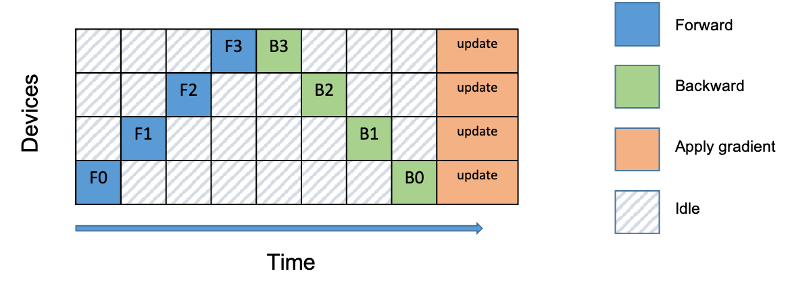
\includegraphics[width=0.85\textwidth]{figure/2-background/mp-time.png}
		\caption{模型并行化}
		\label{fig:mp-time}
	\end{subfigure}
	\begin{subfigure}[b]{0.95\textwidth}
		\centering
		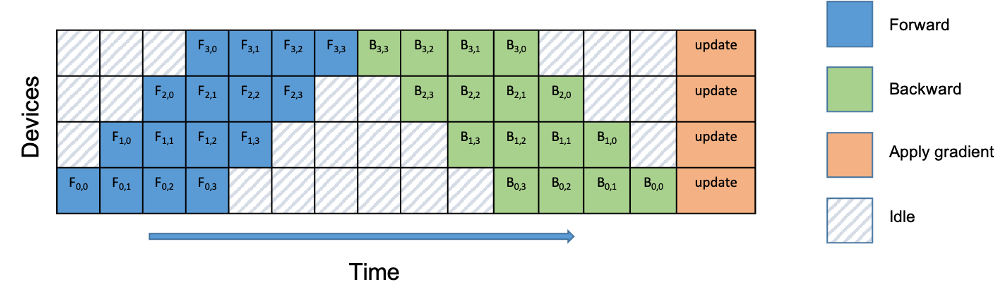
\includegraphics[width=0.85\textwidth]{figure/2-background/gpipe.png}
		\caption{流水线优化}
		\label{fig:gpipe}
	\end{subfigure}
	\caption{模型并行化 vs 流水线并行化}
	\label{fig:mp-gpipe}
\end{figure}

为了缓解模型并行化中,各个设备之间由于相互依赖导致的设备利用率低的问题,Huang等人提出了Gpipe \upcite{gpipe}。
Gpipe使用流水线技术优化模型并行化的过程,如图 \ref{fig:gpipe}所示,对于每个数据批,Gpipe将其进一步细分为微数据批(Micro Batch)。
某个设备处理完当前的微数据批后,将输出发送给下一个设备,然后立刻开始下一个微数据批的处理。
反向传播的过程也是类似,直到一个完整的数据批被处理完成,才更新所有的模型参数。
同时,Gpipe也提出了利用“重计算”优化显存使用。
设备不再暂存当前数据的输出结果,而是在进行反向传播计算梯度时,再重新执行前向传播过程,获取输出,再计算梯度。

除了Gpipe,使用流水线优化模型并行化的工作不断涌现。
Narayanan 等提出了PipeDream \upcite{pipedream}, 一种异步的流水线策略。
在PipeDream中,每个设备上同时维护多个模型参数的版本,当数据批到达时,选用最新的模型参数版本进行训练。
并且在之后的反向传播过程中,也使用相同版本的参数,以保持参数一致性。
Fan等人提出了Dapple \upcite{dapple}。Dapple组合了数据并行化和模型并行化。
模型被划分到多个设备组上,设备组之间使用模型并行化,设备组内部使用数据并行化。
此外Dapple还使用Early Backward技术来节省显存,通过调度每个设备进行前向传播和反向传播的顺序,优先让设备进行当前数据批的反向传播,释放掉中间结果的显存。

本小节中介绍了模型并行化以及在模型并行化上进行优化的一些相关工作。
这些工作主要从模型并行化的计算模式上进行优化,和本文工作\sys{} 中涉及的模型划分是正交的,属于不同的优化方向。
在\ref{sec:partition} 节中,将会介绍有关模型并行化中,进行模型划分的一些相关工作。


\section{模型划分技术}
\label{sec:partition}
% 介绍模型划分技术
% 维度: layer-level和operator level
% 比较,说明operator level粒度细,效果好
% 方向:
% 1. RL 
% 2. 经典算法
% 3. 约束优化
% 4. 启发式

在Gpipe等利用流水线对模型并行化进行优化的工作中,将模型定义为若干连续的层,对模型划分时也是进行以层为单位(Layer-wise)的划分。
尽管按层划分是一种可行的方案,但是其仍有如下的不足:
\begin{itemize}
	\item 限制了使用者定义模型的方式:按层划分只接受可以表示为连续若干层的模型,例如在PyTorch中,这类模型通常定义为\texttt{nn.Sequential},每一层只有一个前驱和一个后继。
	在进行划分时,连续的若干层会被划分到一个设备上。
	然而在实际进行模型开发时,模型并不总是可以表示为连续的若干层,例如一些结构比较复杂的模型,在PyTorch中通常会被定义为 \texttt{nn.Module}。
	而按层划分的方式并不支持对这类模型。
	\item 按层划分难以达到最优的负载均衡:在模型并行化训练中,由于参与训练的设备之间存在依赖关系,因此需要谨慎的划分模型,让不同设备具有近似的负载,来避免负载不均。而层的定义也依赖于开发者,这容易导致层与层之间的大小(参数量、运算量)区别很大,例如在 基于BERT \upcite{bert}的模型中,模型的最后一层占据了整个模型40\%的计算时间,对于这种巨大的层,还需要进一步的划分,才能保证不同设备的负载均衡。
	\item 按层划分是一种粗粒度划分方式:即使模型可以被表示为若干连续的层,那么对这些层进行划分的前提是层数大于设备数目,因为每个设备只少要被分到一层模型,但实际情况不总是如此。
\end{itemize}

在运行时,模型会被执行框架编译为计算图,再由运行时进行执行。
直接对计算图进行划分,也就是按照计算节点划分(Operator-wise) 可以有效避免按层划分的缺点。
从计算图层面对模型进行划分的工作有如下的方向:
\begin{itemize}
	\item \textbf{基于强化学习的方法}:Mirhoseini等提出了基于强化学习的计算图划分方法 \upcite{rl1,rl2}。
	Mirhoseini 使用的模型是NLP领域常用的Seq2Seq \upcite{seq2seq}模型,并在该模型中加入了注意力机制。
	Seq2Seq模型由编码器(Encoder)和解码器(Decoder)两部分组成,编码器和解码器都使用LSTM(Long short-term memory) \upcite{lstm}实现。
	该方法首先将计算图中的每个节点都进行编码,编码内容包括节点的类型,节点的输出大小,节点的邻接表。然后将节点编码序列输入到模型中,由模型输出每个节点的放置结果,也就是节点被放置到的设备编号。
	使用强化学习方法的缺点是需要很长的训练时间。
	\item \textbf{基于任务调度的近似算法}:Jeon等提出了使用基于任务调度的近似算法进行计算图的划分 \upcite{baechi}。
	计算图中的每个节点可以看作具有不同执行时长的任务,设备可以看作运行任务的处理器。
	节点之间的边则定义了任务的依赖,因此,从任务调度的角度,可以将计算图的划分问题建模为在有限个处理器上调度多个具有不同运行时长且具有依赖关系的任务。
	Jeon等使用经典的任务调度近似算法 \upcite{sched}进行计算图的划分,包括最短任务优先(Earliest Task First, ETF) 和最短通信时间(Small Communication Time, SCT) 算法。
	\item \textbf{基于约束优化的方法}:计算图的划分问题在理论上被证明是NP-hard问题 \upcite{sched},因此无法找到多项式时间内的确定性算法对其进行求解,找到给定计算图和给定设备下的最优计算图划分。
	尽管Jeon等提出的近似算法可以快速得到近似解,但是由于算法近似比的限制,往往近似解无法取得和最优解一样的好结果。
	为了能够获得更好的划分结果,Hafeez等 \upcite{pesto}将计算图的划分问题建模为一组约束优化,并使用高性能约束优化器进行求解。
	实验证明,该方法相比于强化学习和近似算法,可以得到更好的划分结果。

\end{itemize}

\section{本章小结}

本章首先对本文中出现的若干术语和概念,如模型、计算图和设备进行了详细的介绍。
然后介绍了分布式深度学习的发展和目前的两种主要模式,包括数据并行化和模型并行化。
有关数据并行化,介绍了其适用场景和主流架构,包括参数服务器架构和All Reduce架构,并对两种架构进行了对比。
有关模型并行化,介绍了模型并行化和数据并行化的区别,以及适用场景,并介绍了对于模型并行化的流水线优化技术。
最后,介绍了模型并行化中一个重要问题,也就是模型的划分问题。比较了分层划分和计算图划分两种方式,并介绍了目前对于模型划分的工作方向。

下一章讲介绍对大型神经网络模型进行训练的难点与挑战,以及我们针对大型神经网络模型训练提出的\sys{}框架的设计。 